% $Header$

\documentclass{beamer}

% This file is a solution template for:

% - Talk at a conference/colloquium.
% - Talk length is about 20min.
% - Style is ornate.



% Copyright 2004 by Till Tantau <tantau@users.sourceforge.net>.
%
% In principle, this file can be redistributed and/or modified under
% the terms of the GNU Public License, version 2.
%
% However, this file is supposed to be a template to be modified
% for your own needs. For this reason, if you use this file as a
% template and not specifically distribute it as part of a another
% package/program, I grant the extra permission to freely copy and
% modify this file as you see fit and even to delete this copyright
% notice. 


\mode<presentation>
{
  \usetheme{Warsaw}
  % or ...

  \setbeamercovered{transparent}
  % or whatever (possibly just delete it)
}


\usepackage[english]{babel}
% or whatever

\usepackage[latin1]{inputenc}
% or whatever

\usepackage{times}
\usepackage[T1]{fontenc}
% Or whatever. Note that the encoding and the font should match. If T1
% does not look nice, try deleting the line with the fontenc.

\begin{document}

\begin{frame}{Problem Identification}
What properties of a borrower make a loan more likely to be fully paid? charged
off?
\begin{enumerate}
\item Context: 
Moneylending is potentially a very lucrative business because many kinds of
business like real estate, etc. leverage money from loans as starting capital.
However, lending money to borrowers unlikely to pay it back is very costly.
\item Criteria for success: When determining whether a loan will be charged off,
\begin{itemize}
\item have a low false positive rate (don't want to deny profitable loans)
\item have a very low false negative rate (want to get paid back)
\end{itemize}
\item Scope of solution space: The focus will be on numerical and categorical
data from information about borrowers and their loan requests. We will be
focusing on loans through Lending Club.
\end{enumerate}
\end{frame}

\begin{frame}{Problem Identification}
\begin{enumerate}
\setcounter{enumi}{3}
\item Constraints within solution space:
\begin{itemize}
\item The data may not be up to date (it is 10 years old)
\item The insights gained may not apply to borrowers in other countries
\end{itemize}
\item Stakeholders to provide key insight:
\begin{itemize}
\item Banks
\item Pawnbrokers
\end{itemize}
\item Key data sources:
data.world dataset about loans issued by lendingclub.com from 2007-2011
with performance data -- contains complete loan data for all loans issued
through the time period stated, including the current loan status (Current,
Late, Fully Paid, etc.) and latest payment information.
\end{enumerate}
\end{frame}

\begin{frame}{Recommendation and key findings}
\begin{itemize}
\item
We are able to determine the four traits most strongly associated with
fully paid loans. They are high mean FICO score, high annual income, 
credit card related purpose, and debt consolidation related purpose.
\item
We are also able to determine the four traits most strongly
associated with charged off loans. They are longer term loans, inquiries
within the last six months, credit utilization rate, and small business
related purpose.
\end{itemize}
\end{frame}

\begin{frame}{Modeling results and analysis}
Logistic regression coefficients for fully paid loans:
\begin{center}
\begin{tabular}{|c|c|}\hline
\texttt{mean\_fico} & $0.378308$ \\\hline
\texttt{annual\_income} & $0.288602$ \\\hline
\texttt{purpose\_credit\_card} & $0.179052$ \\\hline
\texttt{purpose\_debt\_consolidation} & $0.129990$ \\\hline
\texttt{purpose\_car} & $0.083845$ \\\hline
$\vdots$ & $\vdots$ \\\hline
\texttt{loan\_amnt} & $-0.147008$ \\\hline
\texttt{purpose\_small\_business} & $-0.153739$ \\\hline
\texttt{revol\_util} & $-0.155017$ \\\hline
\texttt{inq\_last\_6mths} & $-0.234819$ \\\hline
\texttt{term\_ 60 months} & $-0.383156$ \\\hline
\end{tabular}
\end{center}
\end{frame}

\begin{frame}{Modeling results and analysis}
\begin{center}
Random forest feature importances:
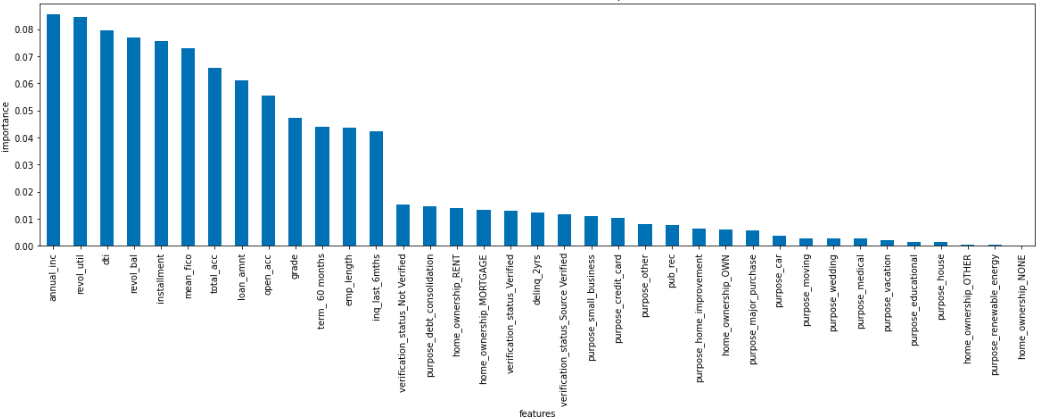
\includegraphics[scale=0.3]{random-forest-feature-importances}
\end{center}
\end{frame}

\begin{frame}{Modeling results and analysis}
\begin{center}
XGBoost feature importances:
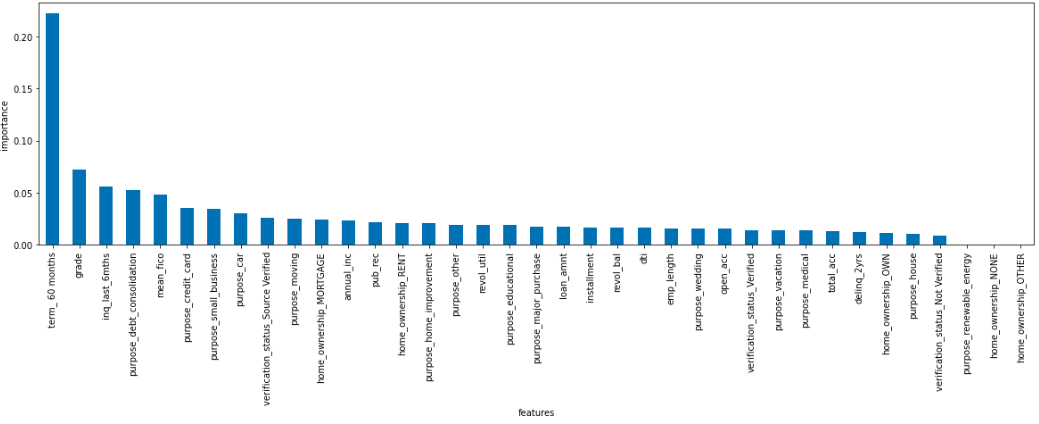
\includegraphics[scale=0.3]{xgboost-feature-importances}
\end{center}
\end{frame}

\begin{frame}{Summary and conclusion}
\begin{itemize}
\item The most creditworthy features are
high mean FICO score, high annual income, 
credit card related purpose, and debt consolidation related purpose.

\item The most subprime features are
longer term loans, inquiries within the last six months,
credit utilization rate, and small business related purpose.

\item Other important features determining loan status are monthly debt to
income ratio, total credit balance, and loan grade.
\end{itemize}
\end{frame}
\end{document}
